\chapter{Cabeçalhos e Rodapés}
\minisec{Usando Estilos de Página Predefinidos}

Uma das características gerais de um documento é o estilo de página. No \LaTeX, isso consiste principalmente no conteúdo dos cabeçalhos e rodapés.
\begin{verbatim}
        headsepline=simple switch
        footsepline=simple switch
\end{verbatim}

Você pode usar essas opções para especificar se uma regra horizontal aparece abaixo do cabeçalho ou acima do rodapé. Você pode usar qualquer um dos valores para interruptores simples mostrados na tabela 2.5, página 41. Definir a opção \texttt{headsepline} como \texttt{true} ou invocá-la sem valor resulta em uma linha abaixo do cabeçalho. Da mesma forma, ativar a opção \texttt{footsepline} resulta em uma regra acima do rodapé. Desativar qualquer uma das opções desliga a respectiva regra.

A opção \texttt{headsepline} naturalmente não tem efeito com os estilos de página vazio e simples, que são descritos abaixo, porque esses estilos dispensam explicitamente um cabeçalho. Tipograficamente, tal linha tem o efeito de fazer o cabeçalho parecer mais próximo do texto. Isso não significa que o cabeçalho precisa ser movido para mais longe do corpo do texto. Em vez disso, o cabeçalho deve ser considerado como pertencente ao corpo do texto para fins de cálculo da área do tipo. O \KOMAScript\ leva isso em consideração ao passar a \texttt{head\-sep\-li\-ne\-op\-tion} para o pacote \textbf{typearea}, que então executa automaticamente a opção de pacote \texttt{headinclude} com o mesmo valor. O mesmo se aplica à linha de separação do rodapé. Ao contrário do \texttt{headsepline}, a opção \texttt{footsepline} também afeta o estilo de página simples porque \textbf{plain} imprime um número de página no rodapé.

O pacote scrlayer-scrpage (veja capítulo 5) oferece mais possibilidades para ajustar linhas em cabeçalhos e rodapés.
\begin{verbatim}
        \pagestyle{page style}
        \thispagestyle{local page style}
\end{verbatim}

\minisec{Geralmente, há quatro estilos de página diferentes:}
\paragraph{empty} é o estilo de página com cabeçalhos e rodapés completamente vazios. No \KOMAScript\ isso é idêntico às classes padrão.

\paragraph{headings} (títulos) é o estilo de página com títulos correntes no cabeçalho. Neste estilo, os títulos são inseridos automaticamente no cabeçalho. Com as classes scrbook e scrreprt, os títulos de capítulos e seções são repetidos no cabeçalho para impressão frente e verso — no lado externo com \KOMAScript no lado interno com as classes padrão. \KOMAScript\ coloca o número da página no lado externo do rodapé; as classes padrão o colocam no lado interno do cabeçalho. Na impressão de um lado, \KOMAScript\ usa apenas os títulos dos capítulos, que são centralizados no cabeçalho, e coloca os números das páginas centralizados no rodapé. scrartcl se comporta de forma semelhante, mas começa um nível mais abaixo na hierarquia de seções, com seções e subseções, porque o nível do capítulo não existe neste caso.

Enquanto as classes padrão convertem automaticamente os títulos correntes em letras maiúsculas, \KOMAScript\ usa a capitalização encontrada nos títulos. Há várias razões tipográficas para isso. Letras maiúsculas são realmente muito grandes como decoração de texto. Se você usá-las de qualquer maneira, elas devem ser definidas um ponto menor e com espaçamento um pouco mais apertado. As classes padrão não levam esses pontos em consideração.

Além disso, as classes \KOMAScript\ suportam regras abaixo do cabeçalho e acima do rodapé com as opções \texttt{headsepline} e \texttt{footsepline} (veja a página 80).

\paragraph{myheadings} corresponde principalmente ao estilo de página de títulos, mas os títulos correntes não são gerados automaticamente --- eles precisam ser definidos pelo usuário. Você pode usar os comandos \verb|\markboth| e \verb|\markright| para esse propósito (veja a página 83).

\paragraph{Plain} é o estilo de página sem cabeçalho e apenas um número de página no rodapé. As classes padrão sempre centralizam esse número de página no rodapé. \KOMAScript\ coloca o número de página no lado externo do rodapé no modo frente e verso. \KOMAScript\ se comporta como as classes padrão na impressão de um lado.

Você pode definir o estilo da página a qualquer momento com a ajuda do comando \verb|\pagestyle|, e essa configuração entra em vigor na próxima página que for gerada. Se você usar \verb|\pagestyle| logo antes de um comando que resulte em uma quebra de página implícita e se o novo estilo de página deve ser usado na nova página resultante, um \verb|\cleardoublepage| logo antes de \verb|\pagestyle| será útil. Mas normalmente você define o estilo da página apenas uma vez, no início do documento ou no preâmbulo.

Para alterar o estilo da página atual apenas, use o comando \verb|\thispagestyle|. Isso ocorre automaticamente em alguns pontos do documento. Por exemplo, o comando
\begin{verbatim}
        \thispagestyle{\chapterpagestyle}   
\end{verbatim}

é emitido implicitamente na primeira página de um capítulo.
Observe que quando você usa o pacote scrlayer-scrpage, alternar entre cabeçalhos automáticos e manuais não é mais realizado alterando os estilos de página, mas com instruções especiais. Você não deve usar os estilos de página \textbf{headings} e \textbf{myheadings} com este pacote.

Para alterar o estilo de fonte usado para o cabeçalho, rodapé ou número de página, use os comandos \verb|\setkomafont| e \verb|\addtokomafont| (veja a seção 3.6, página 58). O mesmo elemento, pageheadfoot, é usado para o cabeçalho e o rodapé. O elemento para o número de página dentro do cabeçalho ou rodapé é chamado pagenumber. O elemento pagefoot, que também é fornecido pelas classes \KOMAScript é usado somente se você definir um estilo de página com o pacote scrlayer-scrpage no qual o rodapé contém texto (veja capítulo 5, página 264).

Você pode encontrar as configurações padrão na tabela 3.8.

\begin{figure}[h]
    \centering
    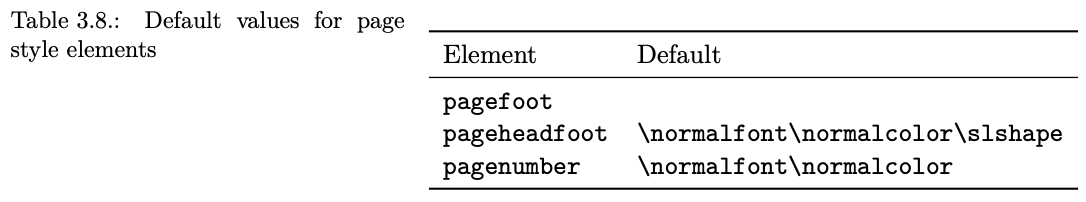
\includegraphics[width=0.8\linewidth]{imagens/tab3_8.png}
    \caption{Tabela 3.8 do Manual}
    \label{fig:tab3_8}
\end{figure}

\begin{verbatim}
        \markboth{left mark}{right mark}
        \markright{right mark}
\end{verbatim}

O estilo de página \textbf{myheadings} não define o cabeçalho de execução. Em vez disso, você o define com a ajuda dos comandos \verb|\markboth| e \verb|\markright|. Dessa forma, a marca da esquerda normalmente será usada no cabeçalho de páginas pares e a marca da direita no cabeçalho de páginas ímpares. Com a impressão de um lado, apenas a marca da direita existe. Com o pacote scrlayer-scrpage, o comando \verb|\markleft| também está disponível.

Você pode usar esses comandos com outros estilos de página também. No entanto, quando combinados com cabeçalhos de execução automáticos, por exemplo, com o estilo de página de títulos, o efeito dos comandos dura apenas até a próxima vez que as respectivas marcas forem definidas automaticamente.
\begin{verbatim}
        \titlepagestyle
        \partpagestyle
        \chapterpagestyle
        \indexpagestyle
\end{verbatim}

\begin{figure}[ht]
    \centering
    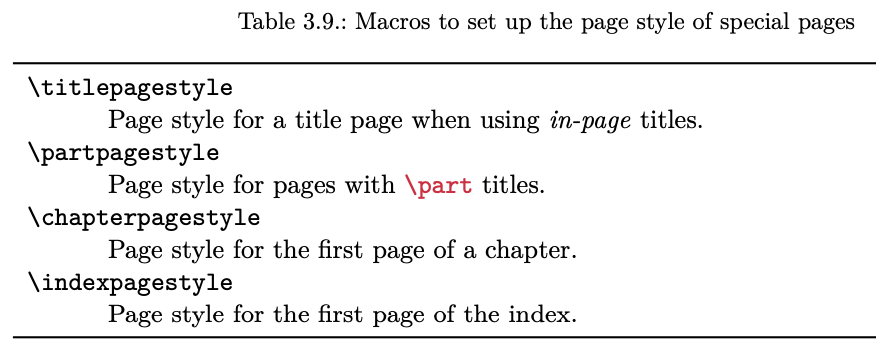
\includegraphics[width=0.75\linewidth]{imagens/tab3_9.png}
    \caption{Tabela 3.9 do Manual}
    \label{fig:tab3_9}
\end{figure}

Em algumas páginas, um estilo de página diferente é escolhido automaticamente com a ajuda do comando \verb|\thispagestyle|. Qual estilo de página realmente é, é definido por essas quatro macros, das quais \verb|\partpagestyle| e \verb|\chapterpagestyle| são encontradas apenas com as classes scrbook e scrreprt, e não em scrartcl. O valor padrão para todos os quatro casos é \textbf{plain}. Você pode encontrar o significado dessas macros  na tabela 3.9. Você pode redefinir os estilos de página com a macro \verb|\renewcommand|.

\textbf{Exemplo}: Suponha que você não queira que as páginas com um título \verb|\part| sejam numeradas. Você pode usar o seguinte comando no preâmbulo do seu documento:
\begin{verbatim}
    \renewcommand*{\partpagestyle}{empty}
\end{verbatim}

Conforme mencionado anteriormente na página 80, o estilo de página vazio é exatamente o que é necessário neste exemplo. Claro, você também pode usar um estilo de página definido pelo usuário.

\minisec{\char`\\\texttt{pagenumbering\{numbering style\}}}

Este comando funciona da mesma forma no \KOMAScript\ como nas classes padrão. Estritamente falando, não é um recurso nem das classes padrão nem das classes \KOMAScript\ mas do kernel \LaTeX. Este comando é usado para alterar o estilo de numeração dos números de página.

As alterações entram em vigor imediatamente, ou seja, a partir da página que contém o comando. Se necessário, você deve primeiro fechar a página atual com \char`\\\texttt{clear\-page} ou melhor \char`\\\texttt{clear\-dou\-ble\-odd\-page}. Você pode encontrar as configurações disponíveis para o estilo de numeração na tabela 3.10.

\begin{figure}[hb]
    \centering
    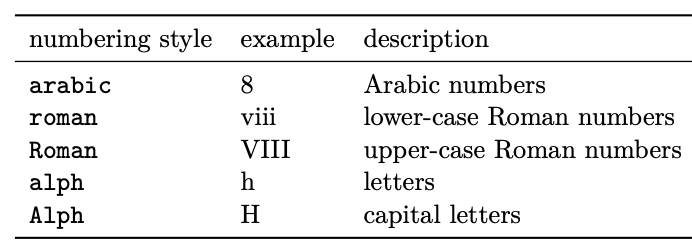
\includegraphics[width=0.7\linewidth]{imagens/tab3_10.png}
    \caption{Tabela 3.10 do Manual}
    \label{fig:tab3_10}
\end{figure}

Chamar \verb|\pagenumbering| sempre redefine o número da página. A página atual se torna o número 1 no estilo de numeração selecionado (\textit{numbering style}). Para que documentos frente e verso produzam os resultados corretos em uma página par, para que a página da esquerda não esteja faltando, você deve sempre adicionar \char`\\\texttt{clear\-dou\-ble\-odd\-pa\-ge} antes de \char`\\\texttt{pa\-ge\-num\-be\-ring}. A próxima seção fornece mais informações sobre páginas em branco potencialmente inseridas.

Deixe-me dizer uma palavra sobre um erro comum encontrado em vários modelos que circulam na Internet. Se você encontrar linhas como a seguinte — sem o comentário inicial, naturalmente — este é um sinal inequívoco de que o criador não leu ou entendeu a observação acima:
\begin{verbatim}
        % Atenção! Este exemplo contém erros!
        % Observe a explicação no texto!
        \tableofcontents
        \pagenumbering{arabic}
        \setcounter{page}{1}
\end{verbatim}

Como \verb|\tableofcontents| gera o índice, mas não emite automaticamente uma quebra de página no final, a numeração de página já foi alterada na última página do índice. Como não tem um comando \char`\\\texttt{clear\-dou\-ble\-odd\-pa\-ge} antes de \char`\\\texttt{pa\-ge\-num\-be\-ring}, ele recebe uma paginação do número arábico 1. Além disso, a linha final que define a numeração de página para 1 é supérflua, pois isso já é feito por \char`\\\texttt{pa\-ge\-num\-be\-ring}.

Às vezes --- sem o comentário inicial, naturalmente --- você encontra:
\begin{verbatim}
        % Atenção! Este exemplo contém erros!
        % Observe a explicação no texto!
        \tableofcontents
        \pagebreak
        \pagenumbering{arabic}
        \setcounter{page}{1}
\end{verbatim}

Aqui, o criador tentou resolver o problema com a página final do índice com a ajuda de \char`\\\texttt{pa\-ge\-break}

Infelizmente, esta solução não é muito melhor. Aqui, há uma quebra de página após a última página do índice. Isso pode fazer com que as entradas na última página de um documento frente e verso tenham espaçamento vertical excessivo (consulte \char`\\\texttt{flush\-bot\-tom}, página 57). \char`\\\texttt{pa\-ge\-break} é claramente o comando errado aqui.

Além disso, \verb|\newpage| ou \char`\\\texttt{clear\-pa\-ge} não seriam suficientes para um documento frente e verso. Por exemplo, se a última página do índice tivesse o numeral romano $vii$, a página direita numerada arábica 1 seguiria imediatamente a página direita numerada romana. Uma página esquerda entre as duas estaria faltando, o que poderia causar sérios problemas com a impressão posterior.

Meu conselho: Evite usar modelos que contenham erros com relação a coisas tão simples. Aliás, a maneira correta seria:
\begin{verbatim}
    \tableofcontents
    \cleardoubleoddpage
    \pagenumbering{arabic}
\end{verbatim}

Isso também se aplica se \textbf{scrartcl} usa uma classe que normalmente não inicia uma nova página após o índice. Se você alternar a numeração de páginas, uma nova página à direita deve ser iniciada. Se você não quiser tal alteração, você deve manter o estilo de numeração das páginas consistente em todo o documento sem alterá-lo entre elas. É mais fácil alterar o estilo de numeração ao usar \textbf{scrbook}. Lá você tem o suporte de dois comandos, \char`\\\texttt{front\-matter} e \char`\\\texttt{main\-matter}, para a alternância mais comumente usada. Para mais informações, consulte a seção 3.15, página 94.
